\documentclass[../psets.tex]{subfiles}

\pagestyle{main}
\renewcommand{\leftmark}{Problem Set \thesection}
\setcounter{section}{2}

\begin{document}




\section{Noncovalent Interactions and Thermodynamics}
\marginnote{11/13:}The questions pertain to the material covered from Noncovalent Interactions (Oct 24) to Isotope Effects (Nov 5).
\begin{enumerate}
    \item The $\pi$-$\pi$ interaction in aromatic systems plays an important role in the fields of chemistry and biology. It affects the crystal packing of organic molecules, molecular recognition processes, and the three-dimensional structures of proteins and DNA.
    \begin{enumerate}
        \item Please use Rowan to complete this question.
        \begin{enumerate}
            \item Using any means, build a molecular model for benzene in Rowan. Then, perform a geometry optimization and charge calculation using the r\textsuperscript{2}SCAN-3c method. Take a screenshot of the webpage before submitting the job and paste it here.
            \begin{itemize}
                \item Note: this job should not take more than 1 minute to run (not including queue time). If
                it takes significantly longer, consider adjusting your initial bond lengths/angles.
            \end{itemize}
            \item Convert the optimized structure into cartesian (XYZ) coordinates and paste them here.
            \item How are the charges distributed on the molecule?
        \end{enumerate}
        \item As mentioned in class, benzene rings can interact through various geometries. Explain why the displaced and T-shaped configurations may exhibit lower energies compared to the sandwich geometry. In your discussion, include considerations of polarization effects and electrostatic interactions.
        \begin{center}
            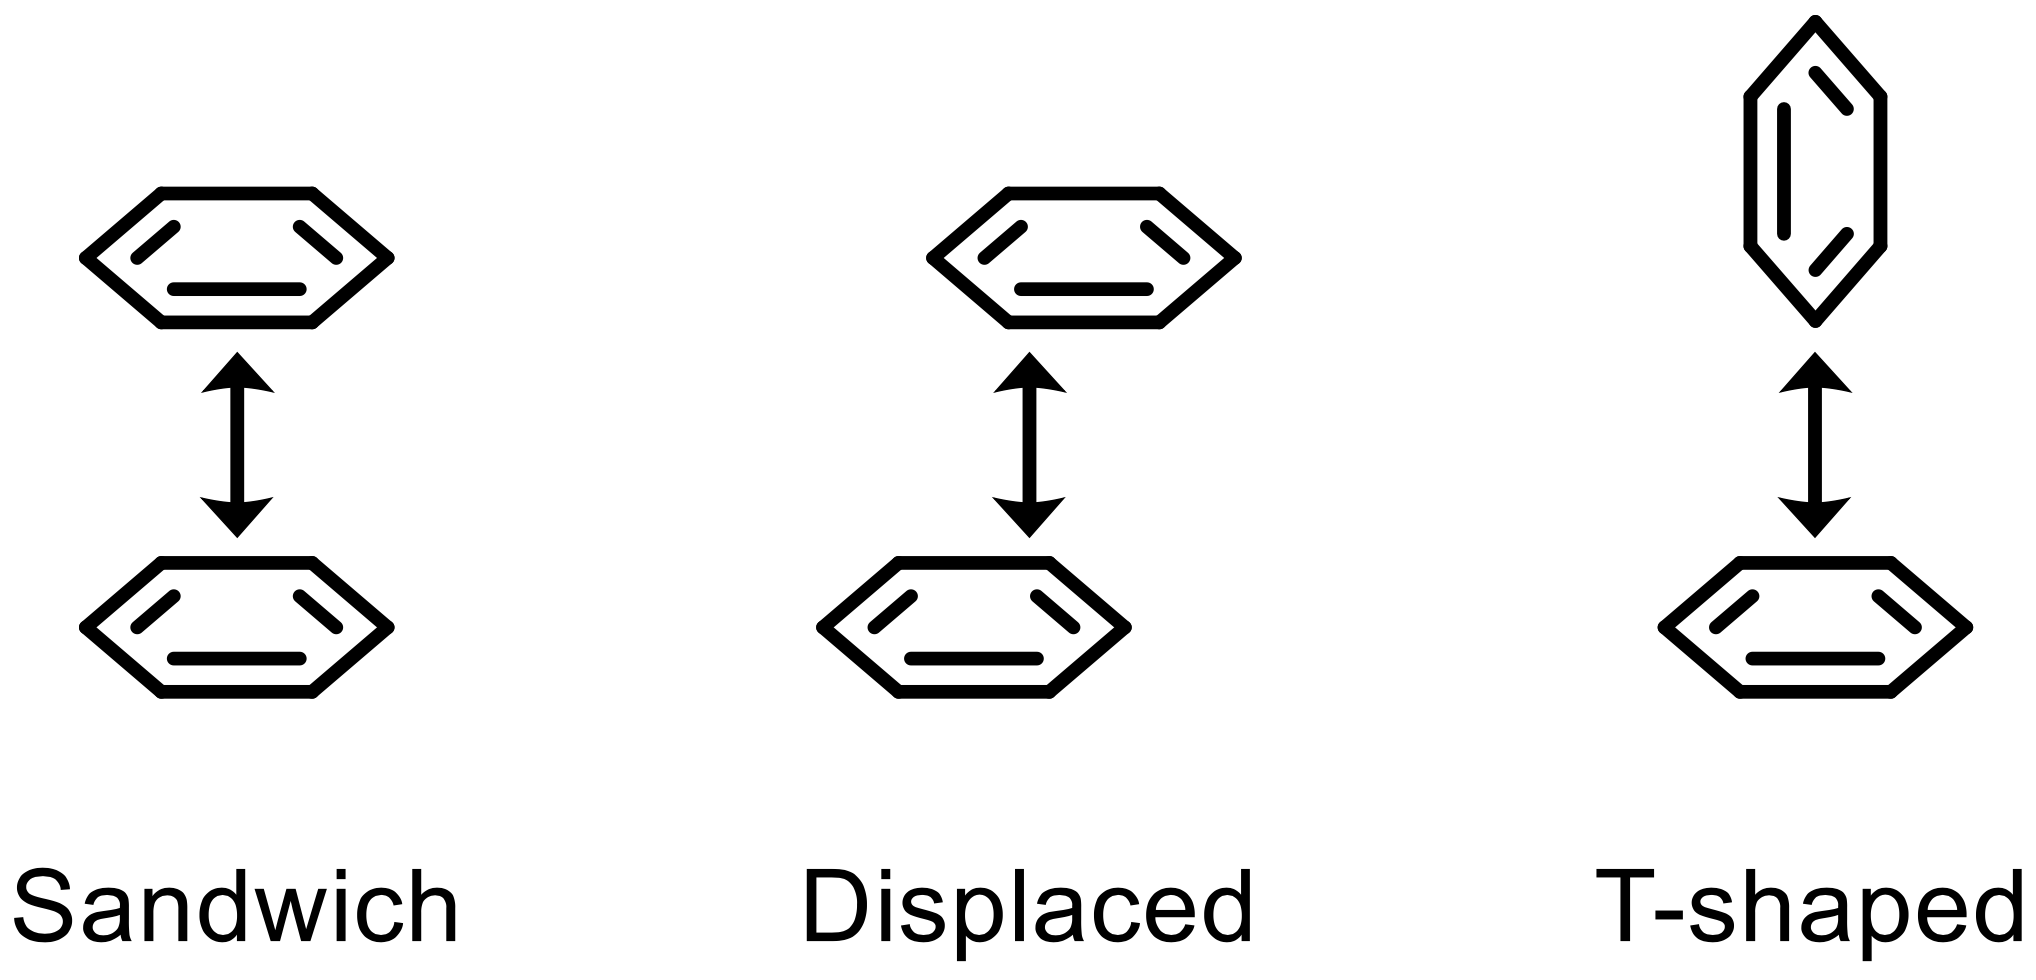
\includegraphics[width=0.4\linewidth]{PSet3F1.png}
        \end{center}
    \end{enumerate}
    \pagebreak
    \item The reaction of dichlorocarbene with isobutylene is known to be one of the exceptions where the reaction has a negative activation enthalpy ($\Delta H^\ddagger$).
    \begin{center}
        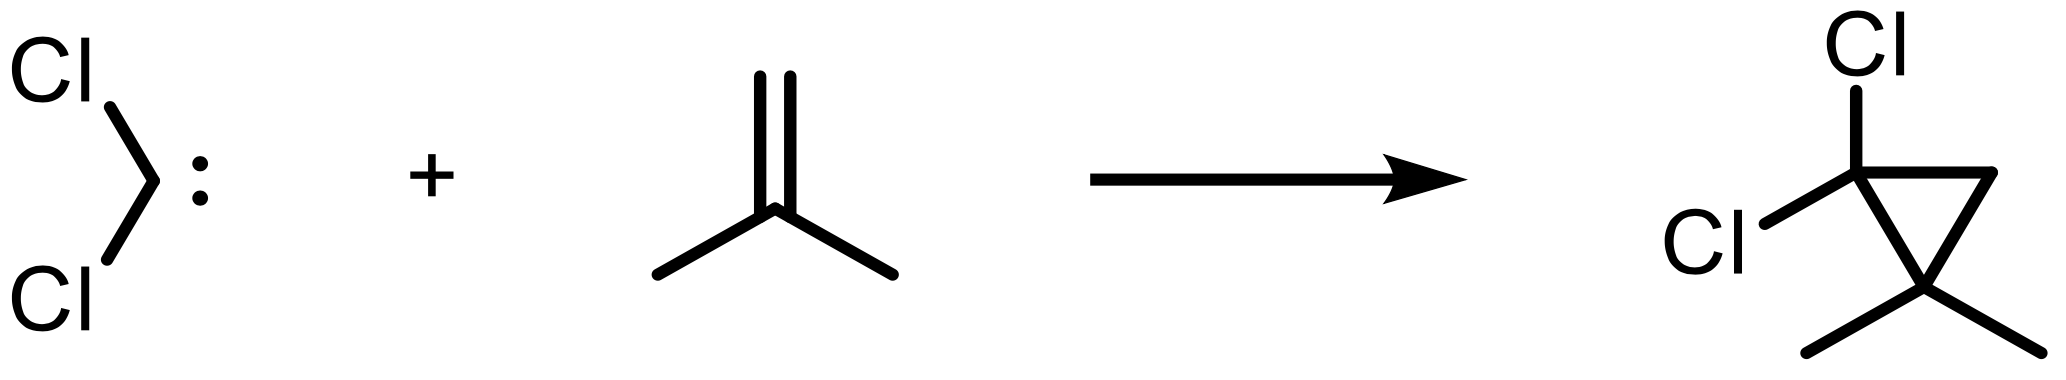
\includegraphics[width=0.4\linewidth]{PSet3F2.png}
    \end{center}
    \begin{enumerate}
        \item Consider the reverse reaction. Conduct a thought experiment in which we gradually pull dichlorocarbene away from isobutylene. How would $\Delta H$ vary with distance? How would $\Delta S$ vary with distance? Draw an energy diagram depicting both $\Delta H$ and $-T\Delta S$ as functions of distance on a single plot. Assume that $\Delta H$ and $\Delta S$ are zero at infinite distance.
        \item If $\Delta H$ dominates at a short distance, and $\Delta S$ dominates at a large distance between the molecules, how would $\Delta G$ change as a function of distance? Draw an energy diagram for $\Delta G$ on the plot from part (a).
        \item Indicate $\Delta G^\ddagger$, $\Delta H^\ddagger$, and $T\Delta S^\ddagger$ on the diagram and explain why this reaction exhibits a negative activation enthalpy.
    \end{enumerate}
    \pagebreak
    \item The following table presents the experimentally measured kinetic data for a Diels-Alder reaction between tetracyanoethylene (TCNE) and 9,10-dimethylanthracene (DMA).
    \begin{center}
        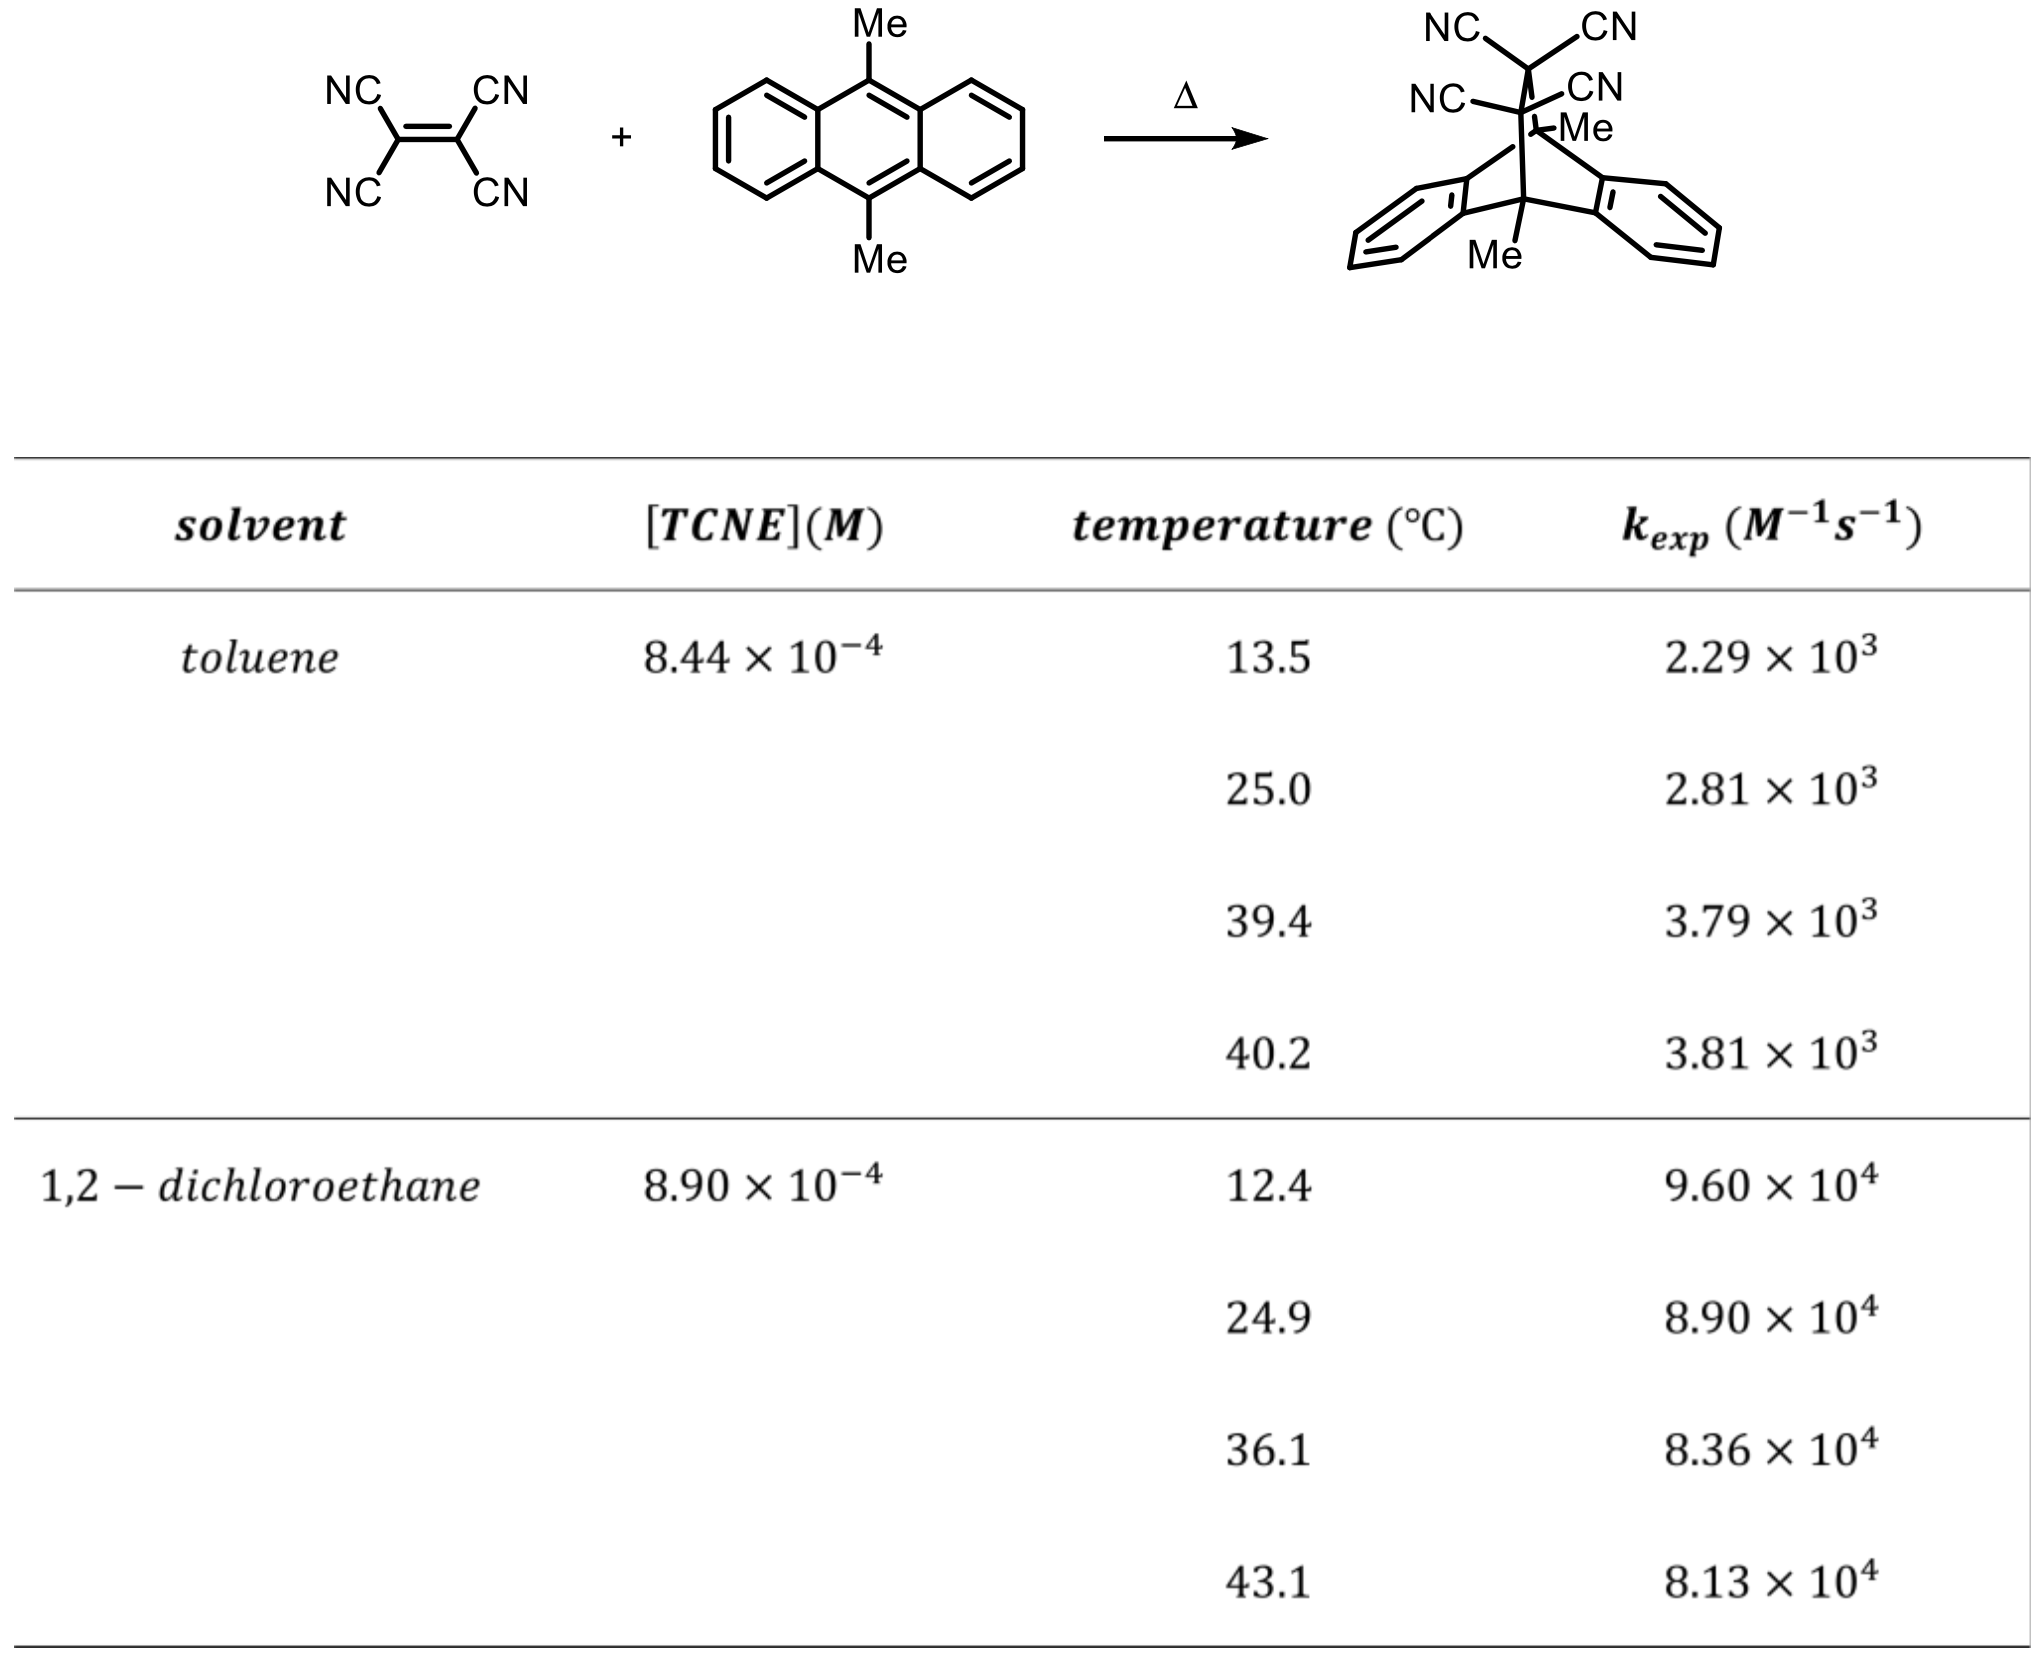
\includegraphics[width=0.8\linewidth]{PSet3F3.png}
    \end{center}
    \begin{enumerate}
        \item Use this data to determine the observed activation enthalpy ($\Delta H^\ddagger$) and activation entropy ($\Delta S^\ddagger$) for the reaction in the following solvents. Use Excel or a similar program to answer the question, and give your answers in units of \si{\kilo\calorie\per\mole} and/or \si{\entropyunit} (\si{\calorie\per\kelvin\per\mole}).
        \begin{enumerate}
            \item Toluene.
            \item 1,2-dichloroethane.
        \end{enumerate}
        \item Considering that $\Delta H^\ddagger$ is positive for most reactions, what is notable about the observed $\Delta H^\ddagger$ value(s) in the above case(s)?
        \item Both experiments and theory support the existence of an intermediate between the starting materials and the product in this reaction, known as an electron donor-acceptor molecular complex. Draw a potential energy diagram with $\Delta H$ (change in enthalpy) on the $y$-axis to rationalize the observed abnormality in part (b).
        \item The mechanism of this reaction is known to be the same in toluene and 1,2-dichloroethane. Based on your answers from part (a) and your energy diagram from part (c), explain how the solvent can make a difference in observed $\Delta H^\ddagger$.
    \end{enumerate}
    \pagebreak
    \item Beak has reported an example of `dynamic thermodynamic resolution' in the asymmetric silylation of benzylic carbanions. In this work, a racemic mixture of dianion \textbf{1} is ligated with 1 equivalent of enantiopure amine \textbf{2} at $-\SI{78}{\celsius}$ to form equal amounts of two new diastereomeric amine-lithium complexes (\textbf{3} and $\bm{3'}$) that have unequal energy. Although the \ce{C-Li} stereocenter in \textbf{3} and $\bm{3'}$ is configurationally stable at $-\SI{78}{\celsius}$, upon warming to $-\SI{25}{\celsius}$, these two complexes readily equilibrate. Upon cooling back to $-\SI{78}{\celsius}$, these anions both react stereospecifically with trimethylsilyl chloride (\ce{TMSCl}) to form enantiomeric products \textbf{4} and $\bm{4'}$. Use this description and the data provided below to answer the following questions. (Equivalents of \ce{TMSCl} are with respect to \textbf{1}).
    \begin{center}
        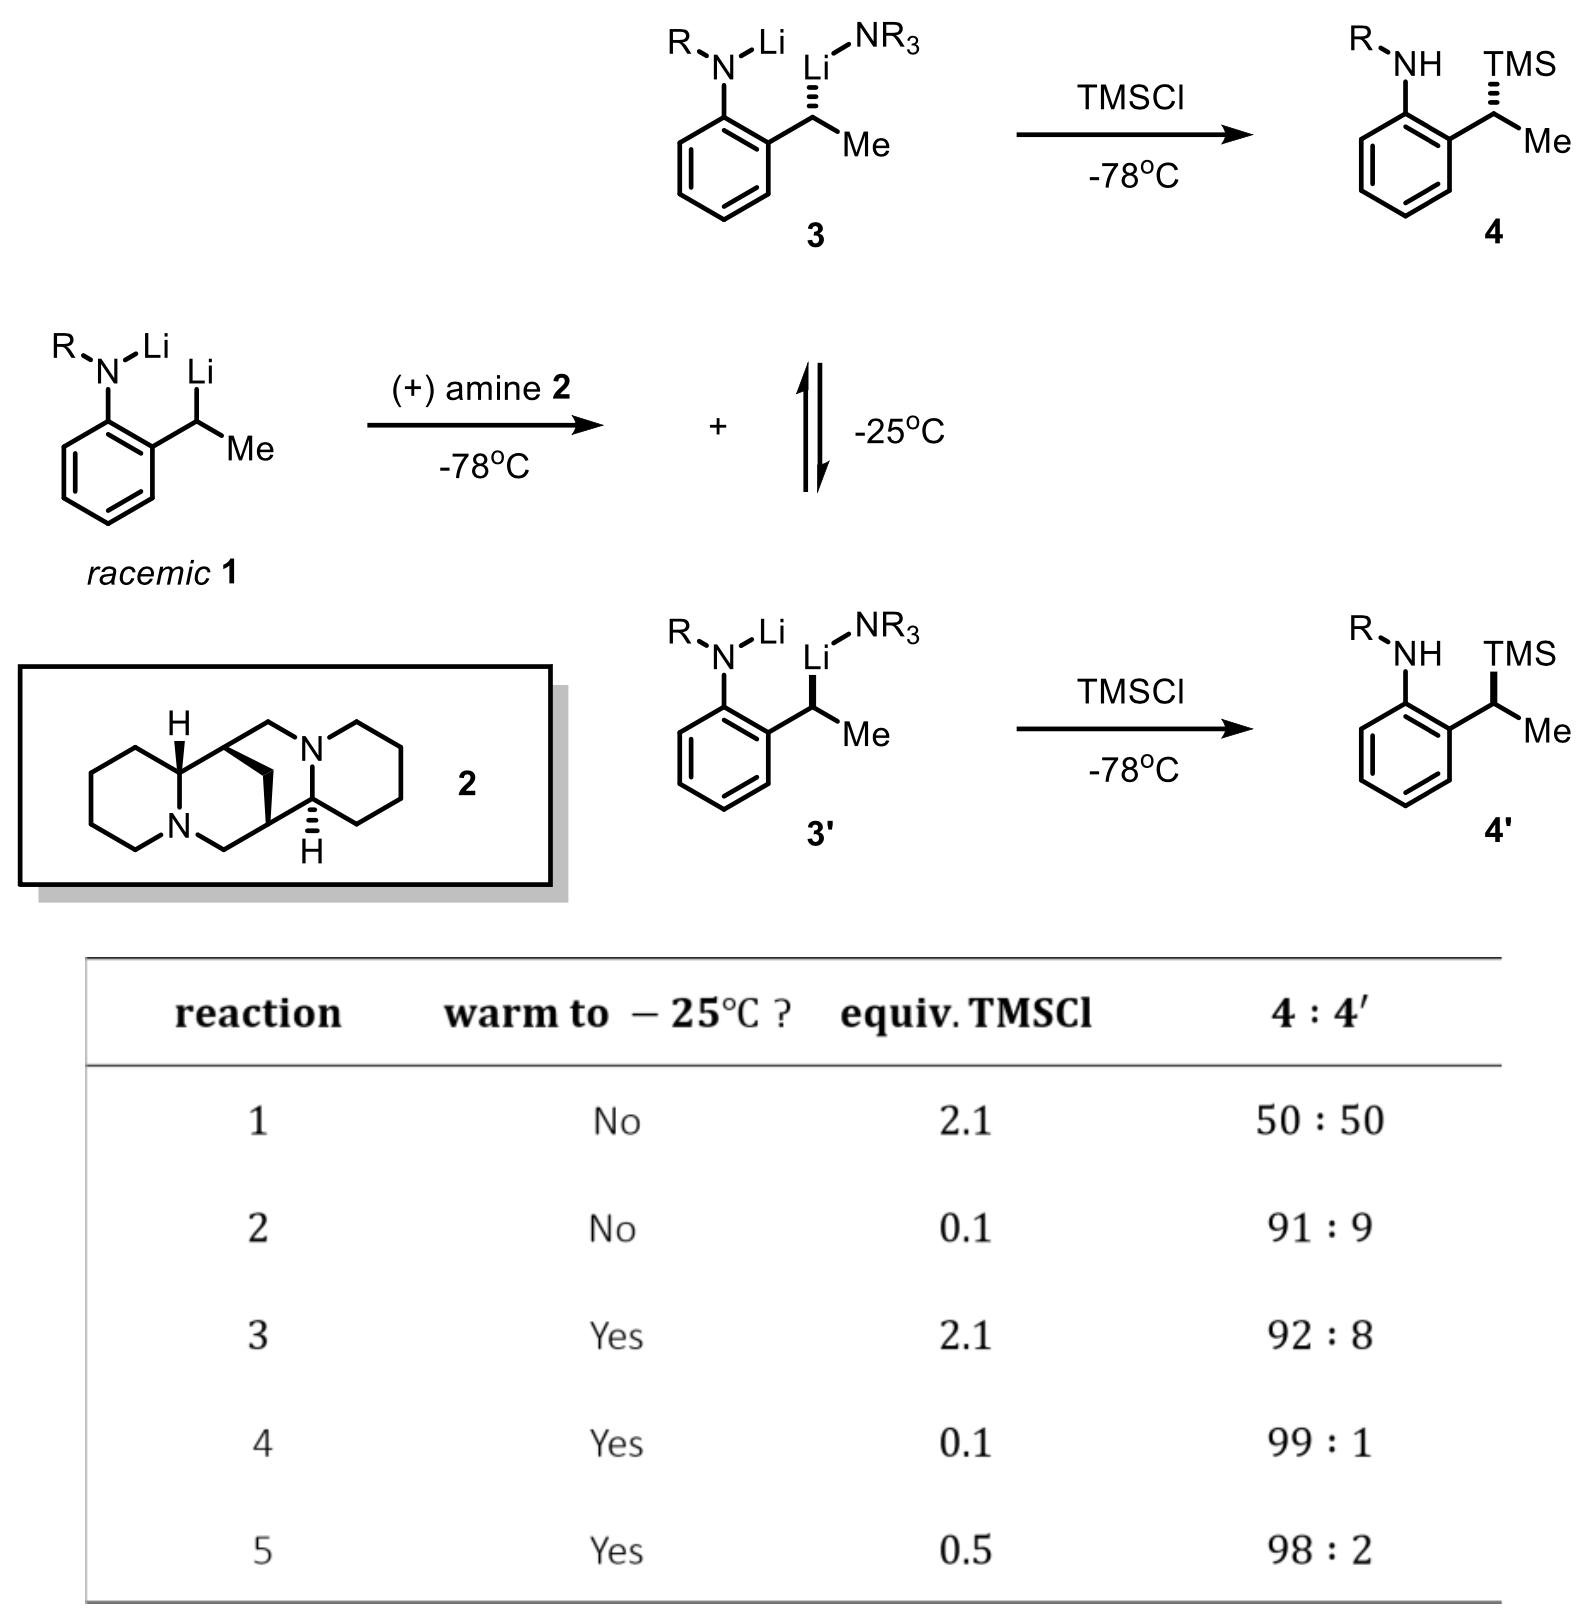
\includegraphics[width=0.8\linewidth]{PSet3F4.png}
    \end{center}
    \begin{enumerate}
        \item Calculate $\Delta G^\circ$ for \textbf{3} and $\bm{3'}$ at $-\SI{25}{\celsius}$.
        \item Calculate $\Delta\Delta G^\ddagger$, for the reactions of \textbf{3} and $\bm{3'}$ with \ce{TMSCl} at $-\SI{78}{\celsius}$.
        \item If one first added 0.5 equiv. of \ce{TMSCl} to an equilibrated mixture of \textbf{3} and $\bm{3'}$, and then subsequently added 2 equiv. of triethylsilyl chloride (\ce{TESCl}), what would be the enantiomeric ratio of the TES-containing products? What would the ratio of TES-containing products be if one first warmed the reaction to $-\SI{25}{\celsius}$ before adding the 2 equiv. of \ce{TESCl}?
        \item Derive expressions to predict the ratio of \textbf{4} and $\bm{4'}$ at both very low conversion ($<1\%$) and at very high conversion ($>99\%$) from an equilibrated mixture of \textbf{3} and $\bm{3'}$. Which elementary step(s) is selectivity-determining in each regime?
    \end{enumerate}
\end{enumerate}




\end{document}